%%%% fatec-article.tex, 2024/03/10

\documentclass[
  a4paper,
  12pt,
  english,
  brazilian,
]{article}

% =========================
% PACOTES
% =========================
\usepackage[]{fatec-article}
\usepackage{float} % Controlar posição das figuras
\usepackage{listings} % Exibir código
\usepackage{xcolor}   % Cores no código

% =========================
% ESTILO PARA SQL
% =========================
\lstdefinestyle{SQLstyle}{
  language=SQL,
  basicstyle=\ttfamily\footnotesize,
  keywordstyle=\color{blue}\bfseries,
  commentstyle=\color{gray},
  stringstyle=\color{teal},
  showstringspaces=false,
  breaklines=true,
  frame=single,
  tabsize=2
}

\begin{document}

\begin{center}
    \large \textbf{\title{ARTEFATOS DO PROJETO DE SOFTWARE}}
\end{center}

\maketitle

\break

\tableofcontents

\break

% =======================================================
\section*{Diagramas UML}
\addcontentsline{toc}{section}{Diagramas UML}

Neste seção serão apresentados os diagramas da UML utilizados para a modelagem do sistema desenvolvido. Dentre os diagramas utilizados, pode-se citar: Diagrama de Caso de Uso, Diagrama de Classe e Diagrama de Objetos.

\subsection*{Diagrama de Caso de Uso}
\addcontentsline{toc}{subsection}{Diagrama de Caso de Uso}

O diagrama de caso de uso mostra os atores do sistema, como Escolas, Professores e Crianças, além de suas funções, como cadastro, envio de planos de aula, atividades personalizadas e acompanhamento do desempenho. Também apresenta o papel da IA na personalização por hiperfoco e correção automática, evidenciando a interação entre usuários e sistema.

\begin{figure}[H]
\centering
\caption{Diagrama de caso de uso}%
\label{fig:diagrama-caso-uso}
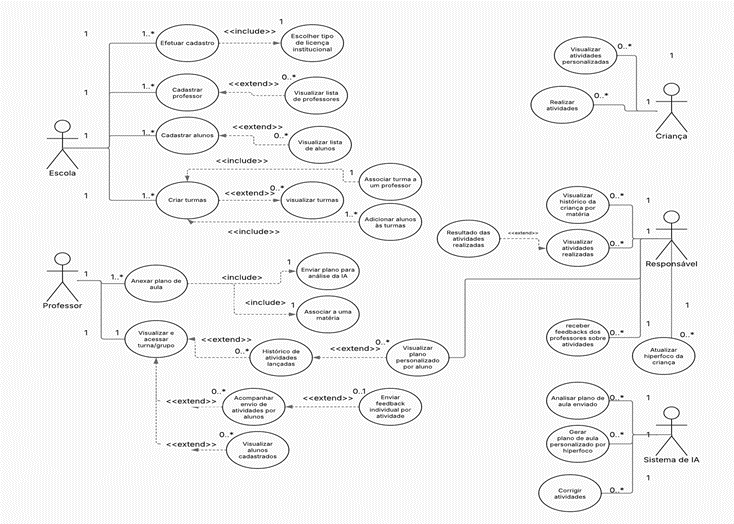
\includegraphics[width=1.1\textwidth]{Logos/caso_de_uso_1.png}
\SourceOrNote{Autoria Própria (2025)}
\end{figure}

Nesse Diagrama é possível observar todos os atores e componentes presentes no sistema, e a relação entre eles. Além de apresentar as funções e ações que cada ator pode realizar.

\subsection*{Diagrama de Classe}
\addcontentsline{toc}{subsection}{Diagrama de Classe}

O diagrama mostra as principais classes do sistema, seus atributos, métodos e relacionamentos. Destacam-se entidades como Usuários, Alunos, Professores, Turmas e Planos de Aula, além das conexões entre elas.

\begin{figure}[H]
\centering
\caption{Diagrama de classe}%
\label{fig:diagrama-classe}
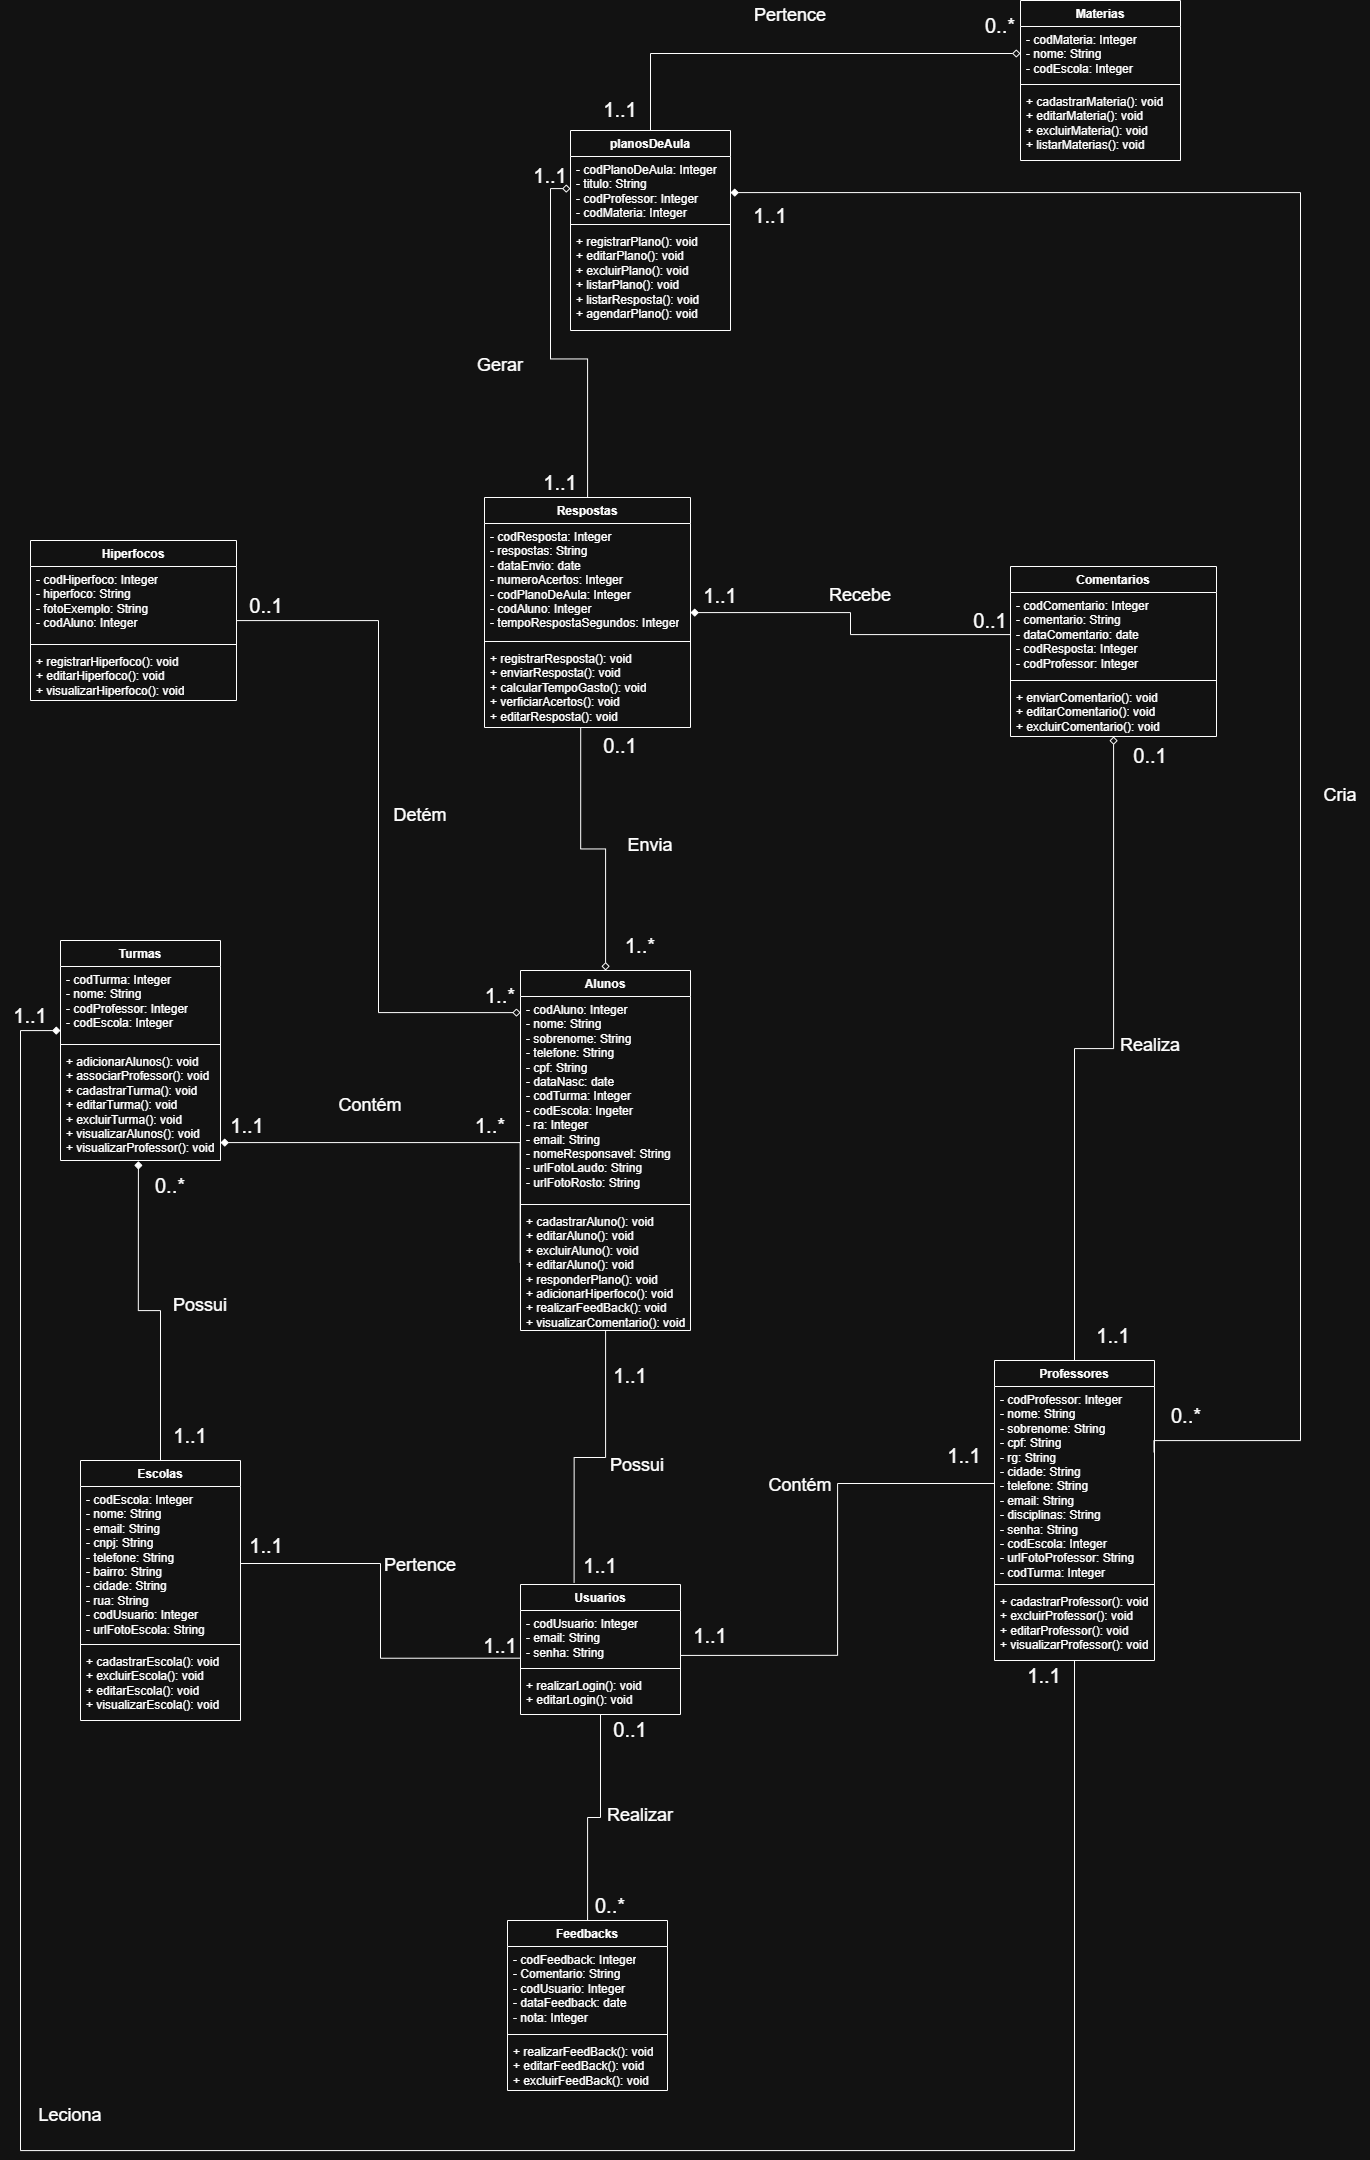
\includegraphics[width=0.8\textwidth]{Logos/diagramaclasse.png}
\SourceOrNote{Autores do projeto (2025)}
\end{figure}

O diagrama apresenta exemplos reais das classes em uso, mostrando como alunos, professores e planos de aula se relacionam na execução do sistema.

\subsection*{Diagrama de Objetos}
\addcontentsline{toc}{subsection}{Diagrama de Objetos}

O diagrama de objetos apresenta instâncias das classes e suas relações no contexto de execução do sistema.

\begin{figure}[H]
\centering
\caption{Diagrama de objetos}%
\label{fig:diagrama-objetos}
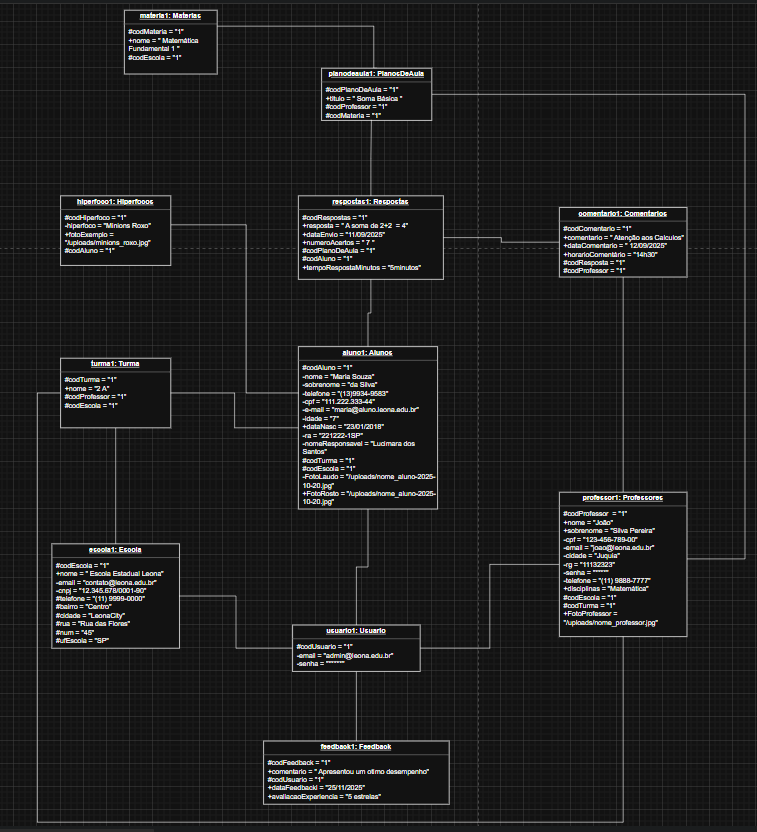
\includegraphics[width=0.8\textwidth]{Logos/diagrama_objetos.png}
\SourceOrNote{Autores do projeto (2025)}
\end{figure}

Ele exemplifica a interação entre elementos como alunos, professores e planos de aula em tempo de execução.

% =======================================================
\section*{Canvas}
\addcontentsline{toc}{section}{Canvas}

Neste trecho será demonstrado o Canvas usado para montar o modelo de negócios do sistema desenvolvido. Permitindo observar os principais componentes do plano de negócios, como proposta de valor, parceiros chaves, canais e relação com o cliente.

\begin{figure}[H]
\centering
\caption{Canvas do projeto}%
\label{fig:canvas}
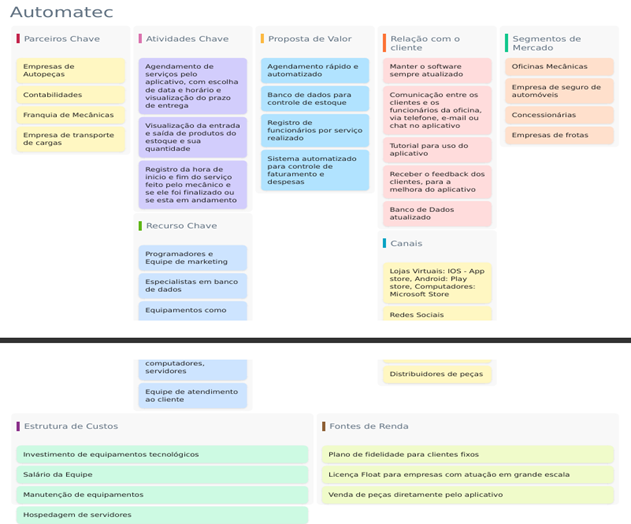
\includegraphics[width=1.0\textwidth]{Logos/canvas.png}
\SourceOrNote{Autores do projeto (2025)}
\end{figure}

A imagem representa nosso modelo de negócios com clientes específicos relacionados ao nosso sistema, a estrutura de custos, o meio como iremos se comunicar com nossos clientes, o diferencial da nossa empresa, etc.

% =======================================================
\section*{Diagrama e Especificações da Infraestrutura da Rede}
\addcontentsline{toc}{section}{Diagrama e Especificações da Infraestrutura da Rede}

Neste tópico será apresentado o Diagrama e Especificações da infraestrutura da rede, utilizado para a demonstração visual da estrutura dos dispositivos interconectados e da conexão com servidores e clientes.

\begin{figure}[H]
\centering
\caption{Diagrama da infraestrutura da rede}%
\label{fig:infra-rede}
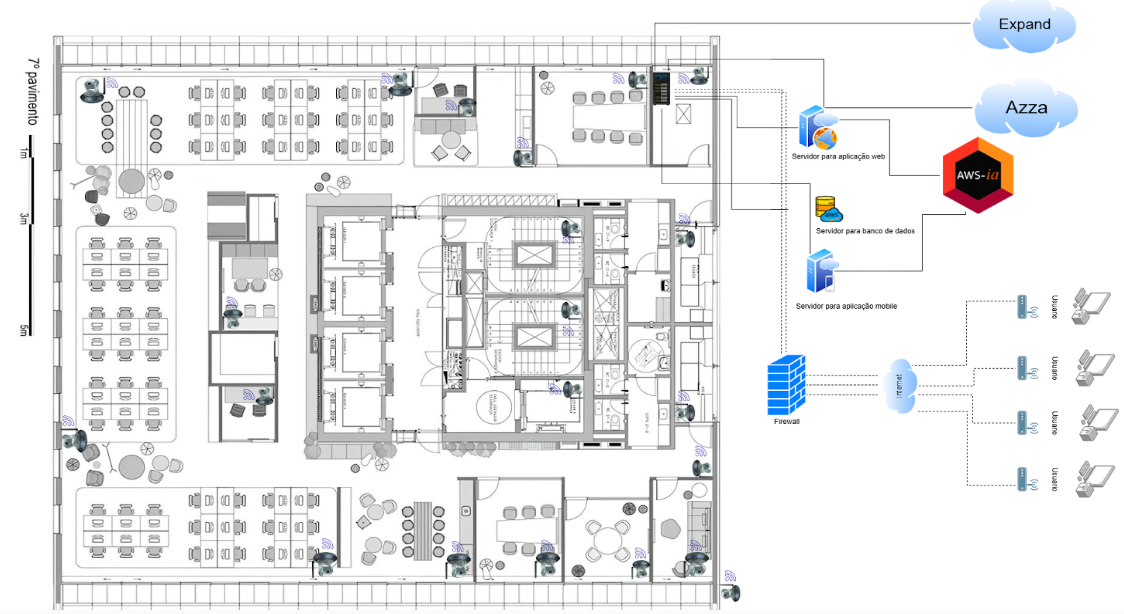
\includegraphics[width=1.0\textwidth]{Logos/infra_rede.png}
\SourceOrNote{Autores do projeto (2025)}
\end{figure}

O Diagrama retrata a empresa e seus dispositivos, podendo observar que os servidores estão em nuvens, como AWS e outras formas de armazenamento, garantindo uma segurança de dados. Percebe-se também o uso de duas conexões com a internet, o que sugere continuidade em caso de falha. E é possível observar a conexão dos servidores da empresa via internet com os usuários.

% =======================================================
\section*{Banco de Dados}
\addcontentsline{toc}{section}{Banco de Dados}

Neste parágrafo será exibido o Diagrama de banco de dados, com todos os objetos e conceitos do mundo real que estão presentes no nosso sistema. Esses diagramas são essenciais para planejar e documentar o banco de dados, facilitando o gerenciamento de informações do sistema. Dentre os bancos de dados temos Conceitual, Lógico e o Script do banco de dados (SQL).

\subsection*{Modelo Conceitual}
\addcontentsline{toc}{subsection}{Modelo Conceitual}

O diagrama conceitual apresenta as principais entidades do sistema, como Professores, Escolas, Crianças e Planos de Aula, bem como seus relacionamentos. Também destaca entidades auxiliares, como Hiperfocos, Feedback e Comentários, que contribuem para o acompanhamento personalizado do desempenho infantil e a gestão educacional.

\begin{figure}[H]
\centering
\caption{Modelo Conceitual}%
\label{fig:modelo-conceitual}
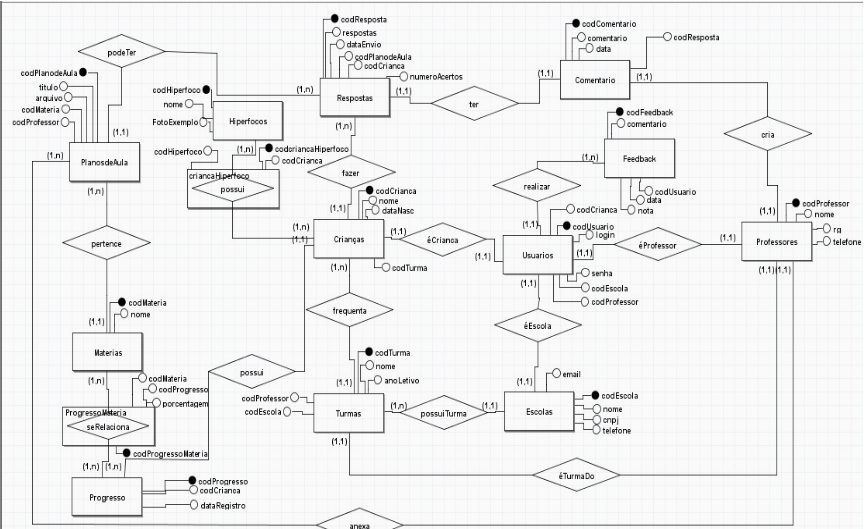
\includegraphics[width=0.9\textwidth]{Logos/modelo_conceitual.png}
\SourceOrNote{Autores do projeto (2025)}
\end{figure}

Esse Diagrama representa as nossas entidades essenciais para o banco de dados e o sistema, os atributos essenciais de cada um e se possuem relacionamento com outra entidade. Caso possuam, é possível observá-las na imagem acima.

\subsection*{Modelo Lógico}
\addcontentsline{toc}{subsection}{Modelo Lógico}

O modelo lógico detalha as estruturas internas do banco, com os atributos de cada entidade e os relacionamentos normalizados. Ele organiza informações como login de usuários, progresso por matéria, hiperfocos associados às crianças e vínculo entre professores, turmas e escolas, garantindo integridade e coerência dos dados.

\begin{figure}[H]
\centering
\caption{Modelo Lógico}%
\label{fig:modelo-logico}
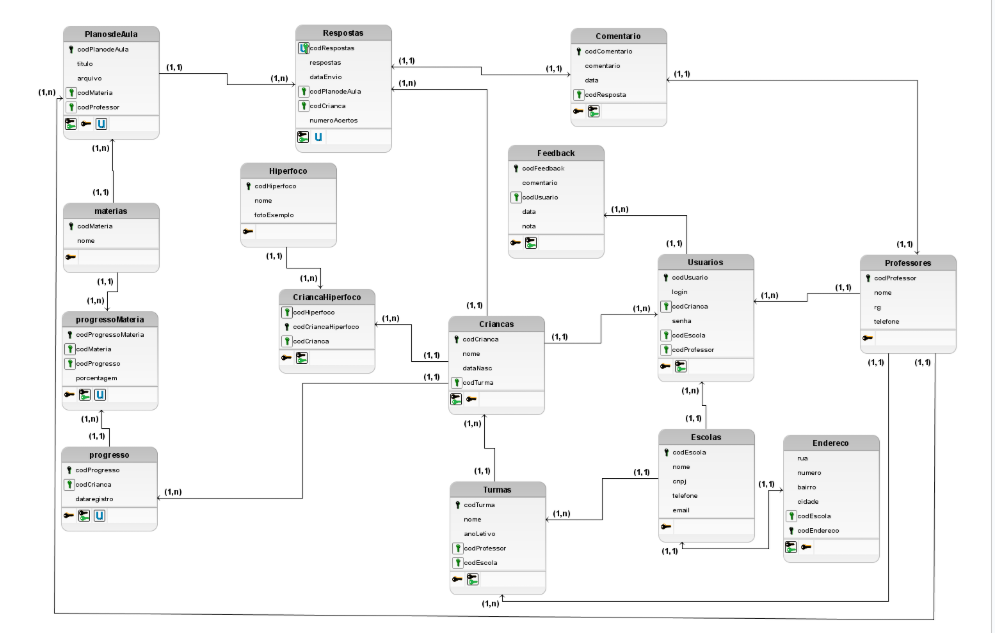
\includegraphics[width=0.9\textwidth]{Logos/modelo_logico.png}
\SourceOrNote{Autores do projeto (2025)}
\end{figure}

O modelo lógico do Diagrama de banco de dados possui as mesmas informações do modelo conceitual. Porém, agora elas são representadas em forma de tabelas.

\subsection*{Script do Banco de Dados (SQL)}
\addcontentsline{toc}{subsection}{Script do Banco de Dados (SQL)}

Nesta subseção é apresentado o código SQL utilizado para a implementação física do banco de dados, conforme os modelos conceitual e lógico definidos anteriormente.

\begin{lstlisting}[style=SQLstyle, caption={Script de criação do banco de dados}]
CREATE DATABASE IF NOT EXISTS projetoIntegrador;
USE projetoIntegrador;


CREATE TABLE usuarios (
    codUsuario INT PRIMARY KEY AUTO_INCREMENT,
    email VARCHAR(100) NOT NULL UNIQUE,
    senha VARCHAR(30) NOT NULL
);

CREATE TABLE escolas (
    codEscola INT PRIMARY KEY AUTO_INCREMENT,
    nome VARCHAR(100) NOT NULL,
    email VARCHAR(100) NOT NULL UNIQUE,
    cnpj VARCHAR(20) NOT NULL UNIQUE,
    telefone VARCHAR(20) NOT NULL,
    bairro VARCHAR(50) NOT NULL,
    cidade VARCHAR(50) NOT NULL,
    rua VARCHAR(50) NOT NULL,
    urlFotoEscola VARCHAR(255) NOT NULL,
    codUsuario INT NOT NULL,
    FOREIGN KEY (codUsuario) REFERENCES usuarios(codUsuario)
);


CREATE TABLE professores (
    codProfessor INT PRIMARY KEY AUTO_INCREMENT,
    nome VARCHAR(100) NOT NULL,
    sobrenome VARCHAR(100) NOT NULL,
    cpf VARCHAR(20) NOT NULL UNIQUE,
    dataNasc DATE NOT NULL,
    rg VARCHAR(20) NOT NULL UNIQUE,
    cidade VARCHAR(50) NOT NULL,
    telefone VARCHAR(20),
    email VARCHAR(100) NOT NULL UNIQUE,
    disciplinas VARCHAR(150) NOT NULL,
    senha VARCHAR(30) NOT NULL,
    urlFotoProfessor VARCHAR(255) NOT NULL,
    codTurma INT,
    codEscola INT NOT NULL,
    FOREIGN KEY (codEscola) REFERENCES escolas(codEscola)
);

CREATE TABLE turmas (
    codTurma INT PRIMARY KEY AUTO_INCREMENT,
    nome VARCHAR(50) NOT NULL,
    codProfessor INT NOT NULL,
    codEscola INT NOT NULL,
    FOREIGN KEY (codProfessor) REFERENCES professores(codProfessor),
    FOREIGN KEY (codEscola) REFERENCES escolas(codEscola)
);


ALTER TABLE professores
ADD CONSTRAINT fk_professores_turmas
FOREIGN KEY (codTurma) REFERENCES turmas(codTurma);

CREATE TABLE alunos (
    codAluno INT PRIMARY KEY AUTO_INCREMENT,
    nome VARCHAR(100) NOT NULL,
    sobrenome VARCHAR(100) NOT NULL,
    telefone VARCHAR(50) NOT NULL,
    cpf VARCHAR(20) NOT NULL UNIQUE,
    dataNasc DATE NOT NULL,
    ra INT NOT NULL,
    email VARCHAR(100) NOT NULL UNIQUE,
    escola VARCHAR(100) NOT NULL,
    urlFotoLaudo VARCHAR(255) NOT NULL,
    urlFotoRosto VARCHAR(255) NOT NULL,
    codTurma INT,
    codEscola INT NOT NULL,
    FOREIGN KEY (codTurma) REFERENCES turmas(codTurma),
    FOREIGN KEY (codEscola) REFERENCES escolas(codEscola)
);

CREATE TABLE feedbacks (
    codFeedback INT PRIMARY KEY AUTO_INCREMENT,
    comentario VARCHAR(300) NOT NULL,
    codUsuario INT NOT NULL,
    dataFeedback DATE,
    nota INT NOT NULL,
    FOREIGN KEY (codUsuario) REFERENCES usuarios(codUsuario)
);

CREATE TABLE materias (
    codMateria INT PRIMARY KEY AUTO_INCREMENT,
    nome VARCHAR (100) NOT NULL UNIQUE,
    codEscola INT NOT NULL,
    FOREIGN KEY (codEscola) REFERENCES escolas(codEscola)
);

CREATE TABLE planosDeAula (
    codPlanoDeAula INT PRIMARY KEY AUTO_INCREMENT,
    titulo VARCHAR(100) NOT NULL,
    codProfessor INT NOT NULL,
    codMateria INT NOT NULL,
    FOREIGN KEY (codProfessor) REFERENCES professores(codProfessor),
    FOREIGN KEY (codMateria) REFERENCES materias(codMateria)
);

CREATE TABLE respostas (
    codResposta INT PRIMARY KEY AUTO_INCREMENT,
    respostas TEXT NOT NULL,
    dataEnvio DATETIME NOT NULL,
    numeroAcertos INT NOT NULL,
    codPlanoDeAula INT NOT NULL,
    codAluno INT NOT NULL,
    tempoRespostaSegundos INT NOT NULL,
    FOREIGN KEY (codPlanoDeAula) REFERENCES planosDeAula(codPlanoDeAula),
    FOREIGN KEY (codAluno) REFERENCES alunos(codAluno)
);

CREATE TABLE comentarios (
    codComentario INT PRIMARY KEY AUTO_INCREMENT,
    comentario VARCHAR(300) NOT NULL,
    dataComentario DATE,
    codResposta INT NOT NULL,
    codProfessor INT NOT NULL,
    FOREIGN KEY (codResposta) REFERENCES respostas(codResposta),
    FOREIGN KEY (codProfessor) REFERENCES professores(codProfessor)
);

CREATE TABLE hiperfocos (
    codHiperfoco INT PRIMARY KEY AUTO_INCREMENT,
    hiperfoco VARCHAR (300) NOT NULL,
    fotoExemplo VARCHAR(200),
    codAluno INT NOT NULL,
    FOREIGN KEY (codAluno) REFERENCES alunos(codAluno)
);
\end{lstlisting}

Este script representa a implementação física completa do banco de dados, incluindo tabelas, chaves primárias e estrangeiras, além das restrições necessárias para garantir a integridade referencial.

\end{document}
